\PassOptionsToPackage{unicode=true}{hyperref} % options for packages loaded elsewhere
\PassOptionsToPackage{hyphens}{url}
%
\documentclass[]{book}
\usepackage{lmodern}
\usepackage{amssymb,amsmath}
\usepackage{ifxetex,ifluatex}
\usepackage{fixltx2e} % provides \textsubscript
\ifnum 0\ifxetex 1\fi\ifluatex 1\fi=0 % if pdftex
  \usepackage[T1]{fontenc}
  \usepackage[utf8]{inputenc}
  \usepackage{textcomp} % provides euro and other symbols
\else % if luatex or xelatex
  \usepackage{unicode-math}
  \defaultfontfeatures{Ligatures=TeX,Scale=MatchLowercase}
\fi
% use upquote if available, for straight quotes in verbatim environments
\IfFileExists{upquote.sty}{\usepackage{upquote}}{}
% use microtype if available
\IfFileExists{microtype.sty}{%
\usepackage[]{microtype}
\UseMicrotypeSet[protrusion]{basicmath} % disable protrusion for tt fonts
}{}
\IfFileExists{parskip.sty}{%
\usepackage{parskip}
}{% else
\setlength{\parindent}{0pt}
\setlength{\parskip}{6pt plus 2pt minus 1pt}
}
\usepackage{hyperref}
\hypersetup{
            pdftitle={Initiating an Experiment},
            pdfauthor={Noushin Nabavi},
            pdfborder={0 0 0},
            breaklinks=true}
\urlstyle{same}  % don't use monospace font for urls
\usepackage{longtable,booktabs}
% Fix footnotes in tables (requires footnote package)
\IfFileExists{footnote.sty}{\usepackage{footnote}\makesavenoteenv{longtable}}{}
\usepackage{graphicx,grffile}
\makeatletter
\def\maxwidth{\ifdim\Gin@nat@width>\linewidth\linewidth\else\Gin@nat@width\fi}
\def\maxheight{\ifdim\Gin@nat@height>\textheight\textheight\else\Gin@nat@height\fi}
\makeatother
% Scale images if necessary, so that they will not overflow the page
% margins by default, and it is still possible to overwrite the defaults
% using explicit options in \includegraphics[width, height, ...]{}
\setkeys{Gin}{width=\maxwidth,height=\maxheight,keepaspectratio}
\setlength{\emergencystretch}{3em}  % prevent overfull lines
\providecommand{\tightlist}{%
  \setlength{\itemsep}{0pt}\setlength{\parskip}{0pt}}
\setcounter{secnumdepth}{5}
% Redefines (sub)paragraphs to behave more like sections
\ifx\paragraph\undefined\else
\let\oldparagraph\paragraph
\renewcommand{\paragraph}[1]{\oldparagraph{#1}\mbox{}}
\fi
\ifx\subparagraph\undefined\else
\let\oldsubparagraph\subparagraph
\renewcommand{\subparagraph}[1]{\oldsubparagraph{#1}\mbox{}}
\fi

% set default figure placement to htbp
\makeatletter
\def\fps@figure{htbp}
\makeatother

\usepackage{booktabs}
\usepackage[]{natbib}
\bibliographystyle{plainnat}

\title{Initiating an Experiment}
\author{Noushin Nabavi}
\date{2020-09-08}

\begin{document}
\maketitle

{
\setcounter{tocdepth}{1}
\tableofcontents
}
\hypertarget{preface}{%
\chapter*{Preface}\label{preface}}
\addcontentsline{toc}{chapter}{Preface}

Welcome to the first edition of initiating an experiment in the public service. I'm so excited to work on this chapter for the experimentation course and work with my vibrant colleagues in the EW2 cohort.

This is a repository to house course materials related to module 2 of Government of Canada's Experimentation Course: \emph{Initiating an Experiment: what do you need to consider before starting an experimental project?}

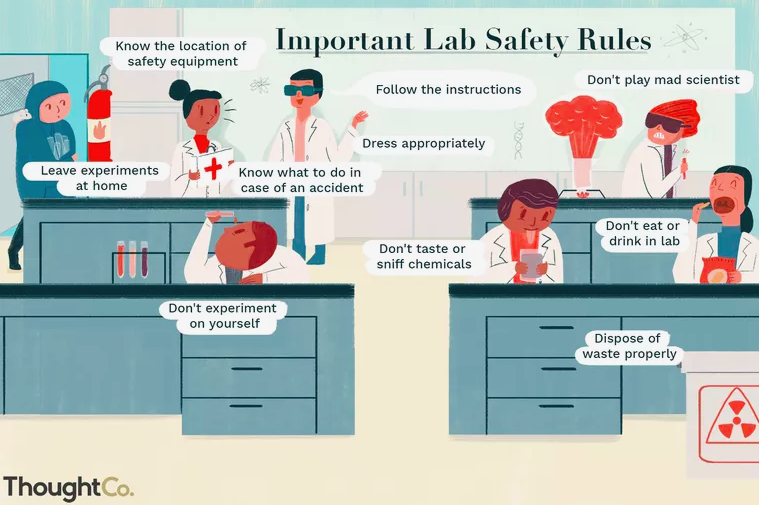
\includegraphics{fig/experimentation-rules.png}

I hope this resource will be useful in clarifying \textbf{when} to experiment, \textbf{what} experiments are useful and \textbf{why}, \textbf{which} pitfals to consider, as well as simplifying scientific and technological jargon and common misperceptions. As innovators seeking social good, we have a duty to put our ideas to test and discover what doesn't work, what does, and find out how to improve people's lives.

I am tremendously grateful for the mentorship I have received from the EW2 leading team (Pierre-Olivier Bedard, Dan Monafu, and Sarah Chan) as well as the graphical design work lead by Jordana Globerman.

I will appreciate to know how this course can be improved and what additional topics can be added. I also love to hear how public servants foresee using the experimentation concepts in their projects towards evidence-based transformation of policies, programs, and services.

A big thanks to Preet Chauhan, EW2 expert, for proof-reading and helping with the many examples.

\hypertarget{prerequisites}{%
\section{Prerequisites}\label{prerequisites}}

This course is intended for anyone with a curiosity and interest in making scientific observations through experimentation, and does not require previous experience of studying the subject.

An interest in experimentation, willingness to experiment, and an apetite for informed consumation of evidence. It means admitting that we don't know all the answers but we can put our ideas to test.

Experimentation also necessitates a more mature attitude from leaders and decision-makers, one that is willing to experiment and learn positively from ``good failure'' rather than pretending we have all the answers.

A team of knowledgeable partners with expertise in experimentations methodologies with a transparent and ``open-by-default'' approach.

\hypertarget{themes}{%
\section{Themes}\label{themes}}

We will explore the following themes in this module to help us answer the question of what we need to consider before starting an experiment: (1) opportunities to experiment in government, and (2) designing experiments as part of existing programs/services.

\hypertarget{learning-objectives}{%
\section{Learning objectives}\label{learning-objectives}}

By the end of this module, you will be able to:

\begin{itemize}
\tightlist
\item
  Identify the steps needed before starting an experimental project
\item
  Devise a problem statement for the project and design a research experiment
\item
  Apply experimentation knowledge to specific examples, cases and scenarios
\end{itemize}

\hypertarget{outline}{%
\section{Outline}\label{outline}}

\begin{longtable}[]{@{}ll@{}}
\toprule
Chapter & Title\tabularnewline
\midrule
\endhead
1 & Before initiating an experiment\tabularnewline
2 & Components of an experimental project\tabularnewline
3 & Mechanics of endorsement\tabularnewline
4 & Case studies\tabularnewline
5 & References\tabularnewline
\bottomrule
\end{longtable}

\hypertarget{before-starting-an-experiment}{%
\chapter{Before starting an experiment}\label{before-starting-an-experiment}}

\hypertarget{do-we-need-to-experiment}{%
\section{Do we need to experiment?}\label{do-we-need-to-experiment}}

To embark on an \texttt{experimentation\ project}, we really need to consider whether an \emph{experimentation} is needed in the first place. One way of determining this is to consider whether out of the many questions that a team has come up with, are there any that require a specific answer to a very specific question? And is the answer worthy to know? If we are after questions that are not causal in nature, then an experiment is likely not the best fit.

At this point in the \textbf{experimentation cycle}, there are more questions than answers and the more questions one asks, the more clarifying answers one will seek on whether an experiment is really needed.

\emph{What would experimentation look like in policy or practice? why would an experiment be worth investing in? what data or program performance tracking is already in place? what experimental tools are available and whether and when they might fall short? what are the risks? What could be a risk management strategy?}

\textbf{Decision tree}

To help make whether an experiment is needed and set one's direction, the following decision tree from Nesta is a great starting point for a project journey. In this journey, only the two red bubbles refer to an experiment. The rest are only explorations or validations.
What makes the two red bubbles an experiment? what do they have in common?

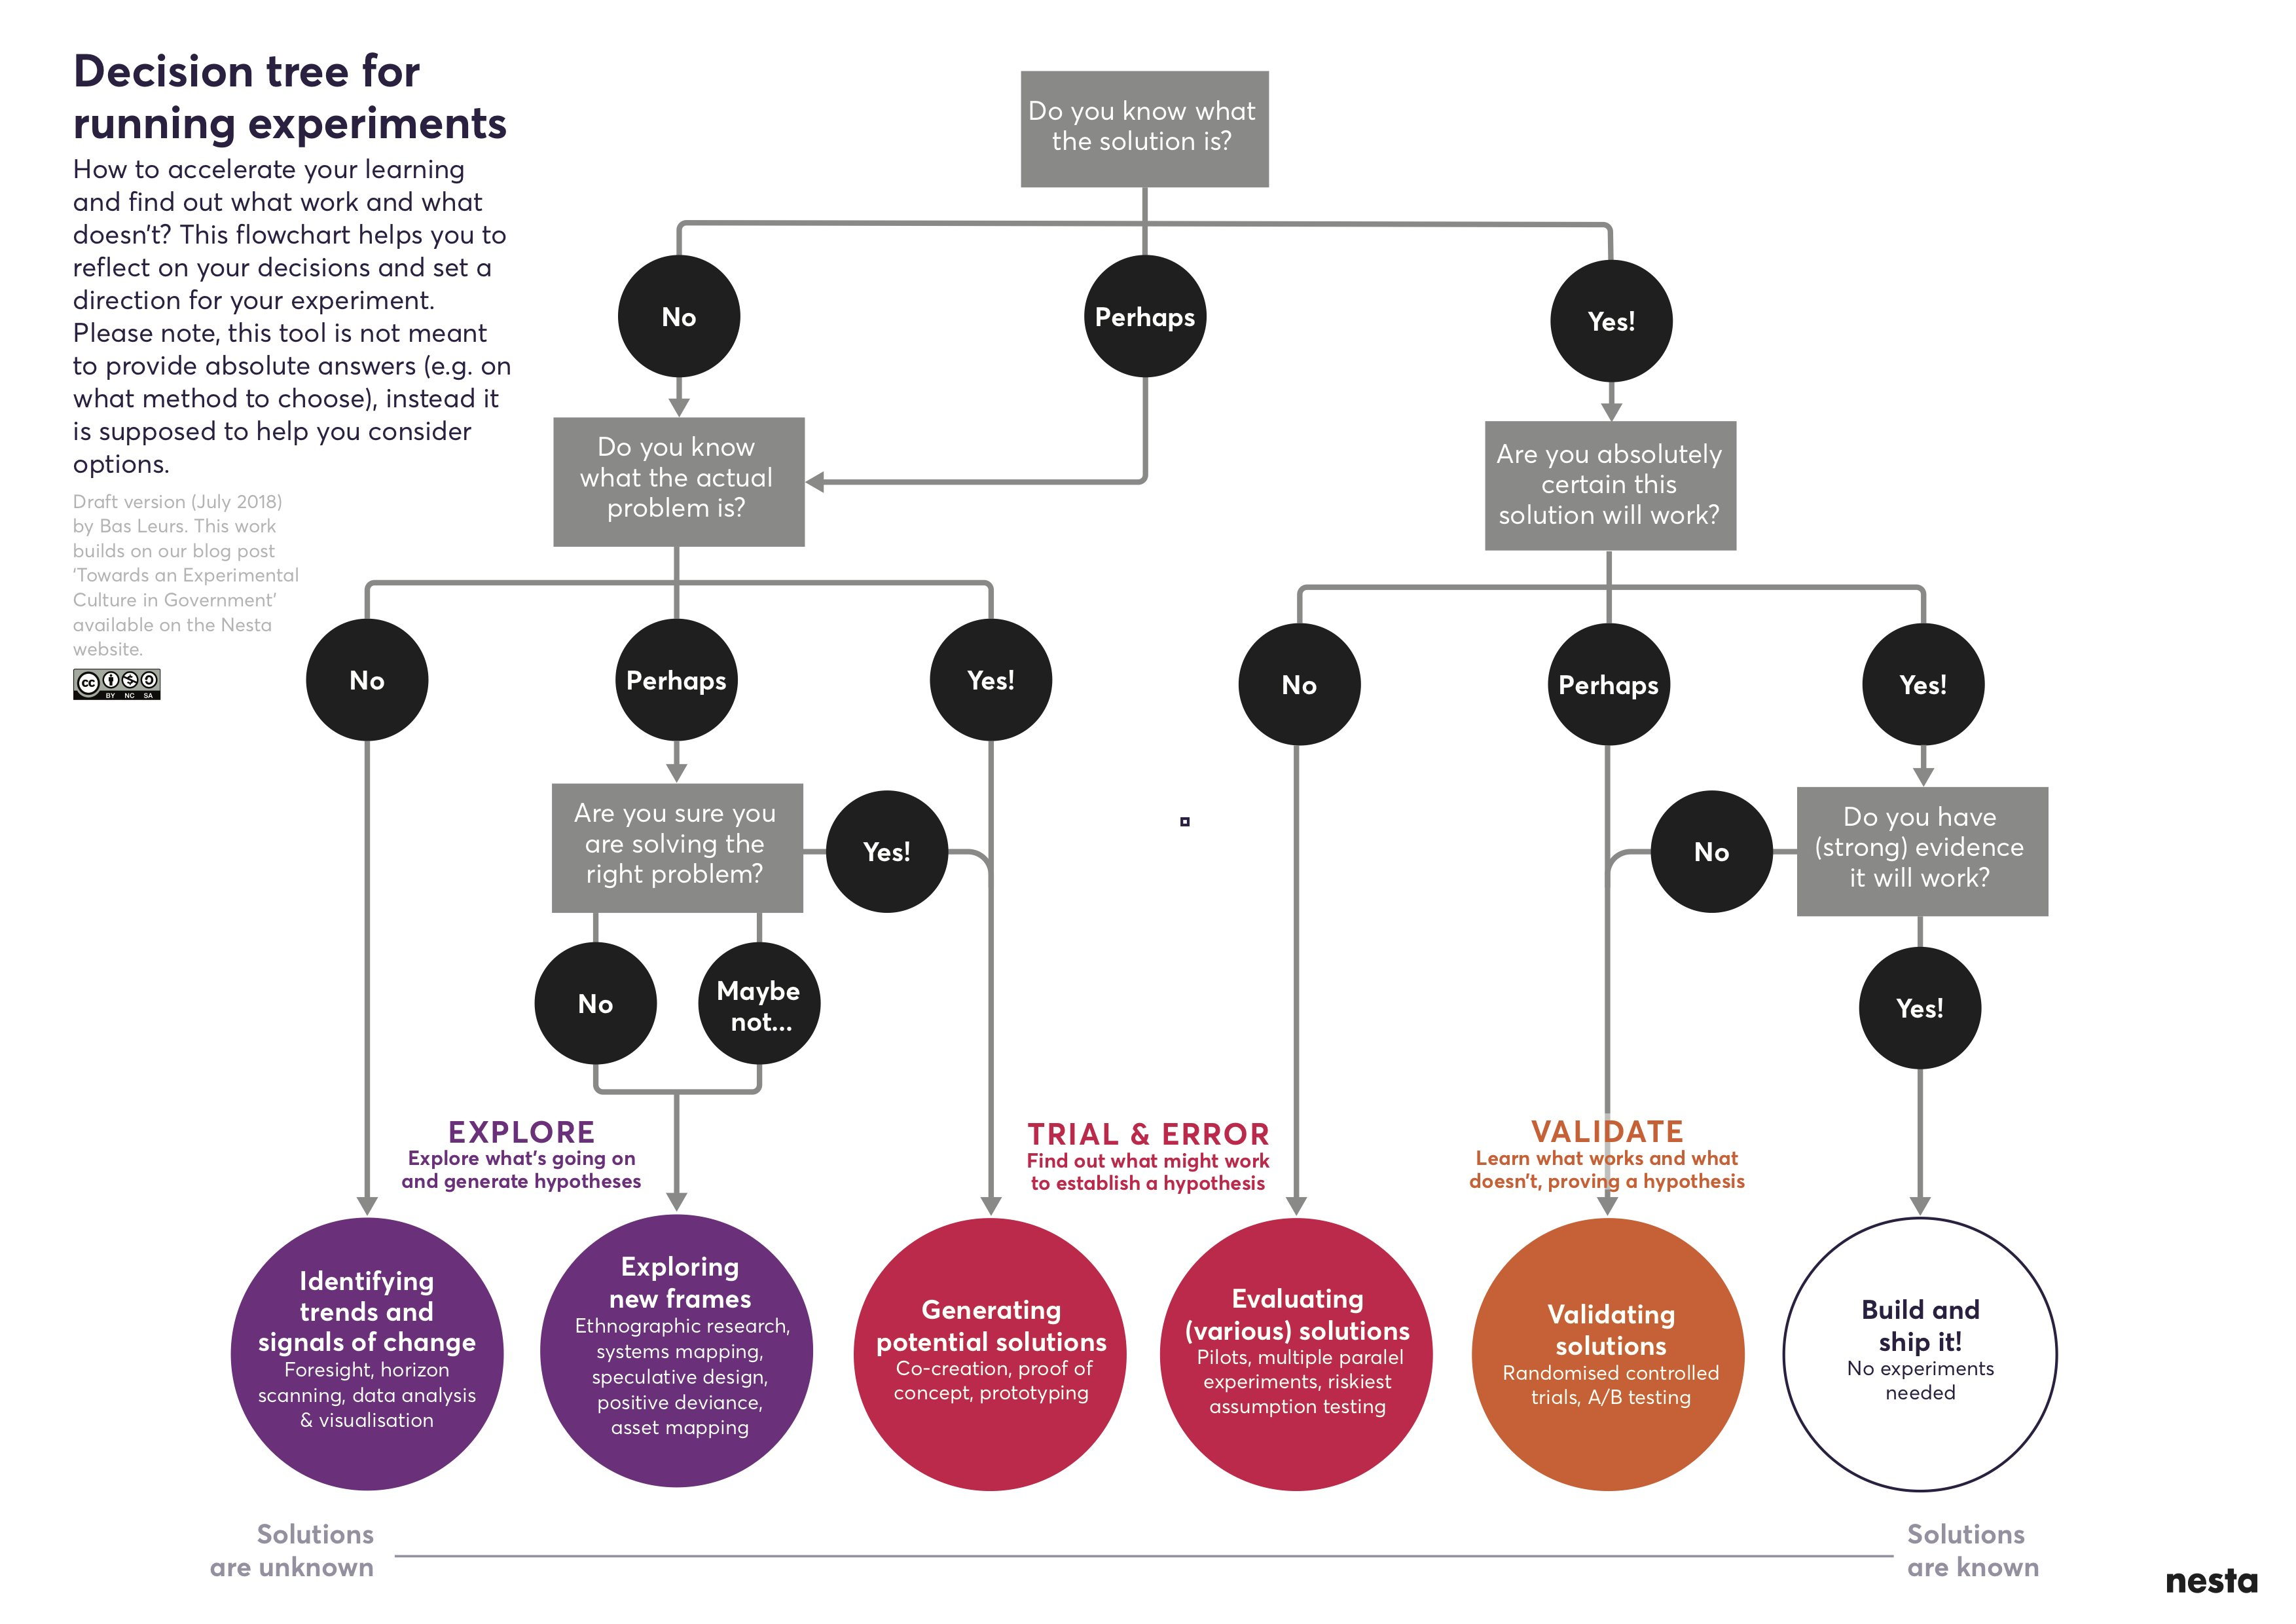
\includegraphics{fig/decision_tree.jpeg}

\hypertarget{the-experimentation-cycle}{%
\section{The experimentation cycle}\label{the-experimentation-cycle}}

\begin{quote}
A problem well-stated is half-solved!
\end{quote}

To help others understand the problem as we see it, the question needs to be well framed and the goals clearly articulated. To help formulating the \texttt{why} as well as the \texttt{what}, the following experimentation lifecycle is helpful in that it encourages to reiteratively (1) brainstorm and form vague ideas, (2) group vague ideas, (3) make general observations, (4) hypothesize, (5) determine a model/method to test the hypotheses, (6) do the experiment to test hypothesis, (7) gather data, analyze, and interpret the results, and (8) learn and communicate learnings to stakeholders

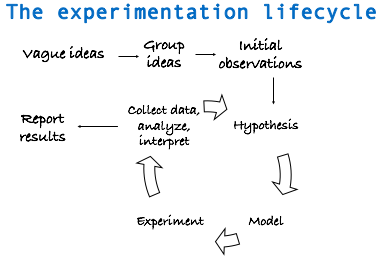
\includegraphics[width=0.8\textwidth,height=\textheight]{fig/experiment_lifecycle.png}

This lifecycle presumes that we can:

\begin{itemize}
\tightlist
\item
  sketch out what information we need to collect (or already have) to get from a vague idea to the hypothesis stage for a planned project
\item
  get invested in the problem before the solution nor in a particular result (any biases will work against us here)
\item
  not get stuck in a fishing expedition (i.e.~grouping ideas forever)
\item
  understand the problem well enough to crisply articulate the goals, questions, and hypotheses before building metrics.
\item
  select metrics that will help answer the questions. This can include system parameters, workload parameters, behaviours, etc. \texttt{“If\ all\ you\ have\ is\ a\ hammer,\ everything\ looks\ like\ a\ nail.”\ -\ Bernard\ Baruch}
\item
  identify parameters that affect behaviour or observations and decide which parameters or interactions to study, or vary.
\end{itemize}

\hypertarget{what-can-go-wrong}{%
\section{What can go wrong?}\label{what-can-go-wrong}}

\begin{quote}
Don't land your plane in forests, and don't do experimental designs before you have considered its drawbacks
\end{quote}

Every positive side comes with a negative one, and so no design is really perfect. This is not to discourage us. In a way, George Box's (British statistician) quote that ``All models are wrong, but some are useful'' applies to experimental designs as well. One single experimental design cannot be comprehensive and all-encompassing. Additionally, we cannot control for the many factors and behaviours that may affect a situation.

Therefore, since all models are wrong, researchers should check the scope of applicability and limitations of their method/model. We should choose the designs that best answer a research question, and not try to tailor the research question to the method at hand.

For instance, we may decide to base our tests on a set of observations derived from survey findings and not be aware that survey data can badly fail in several aspects:
(1) people act differently when they realize they are under study. If asked about questions on sensitive topics (e.g., homosexuality, immigration, abortion, or Donald Trump), people understand there is a ``standard'' answer and so, they may hide their true feelings and give socially acceptable answers.
(2) having a representative sample is difficult and expensive. In social sciences, one of the basis of experiments is recognizing regional diversity (e.g.~British Columbia is different from Ontario and Ontario is different from Quebec). This can affect the interpretation of our findings and their generalizability.
(3) determining the causal relations between two events is usually the goal of experimentation. However, direction of causal inference in social situations can be problematic. Traditional quantitative methods are particularly ill-designed for causal questions when the answer can go in either directions. A solution here is a carefully designed experiment with control groups

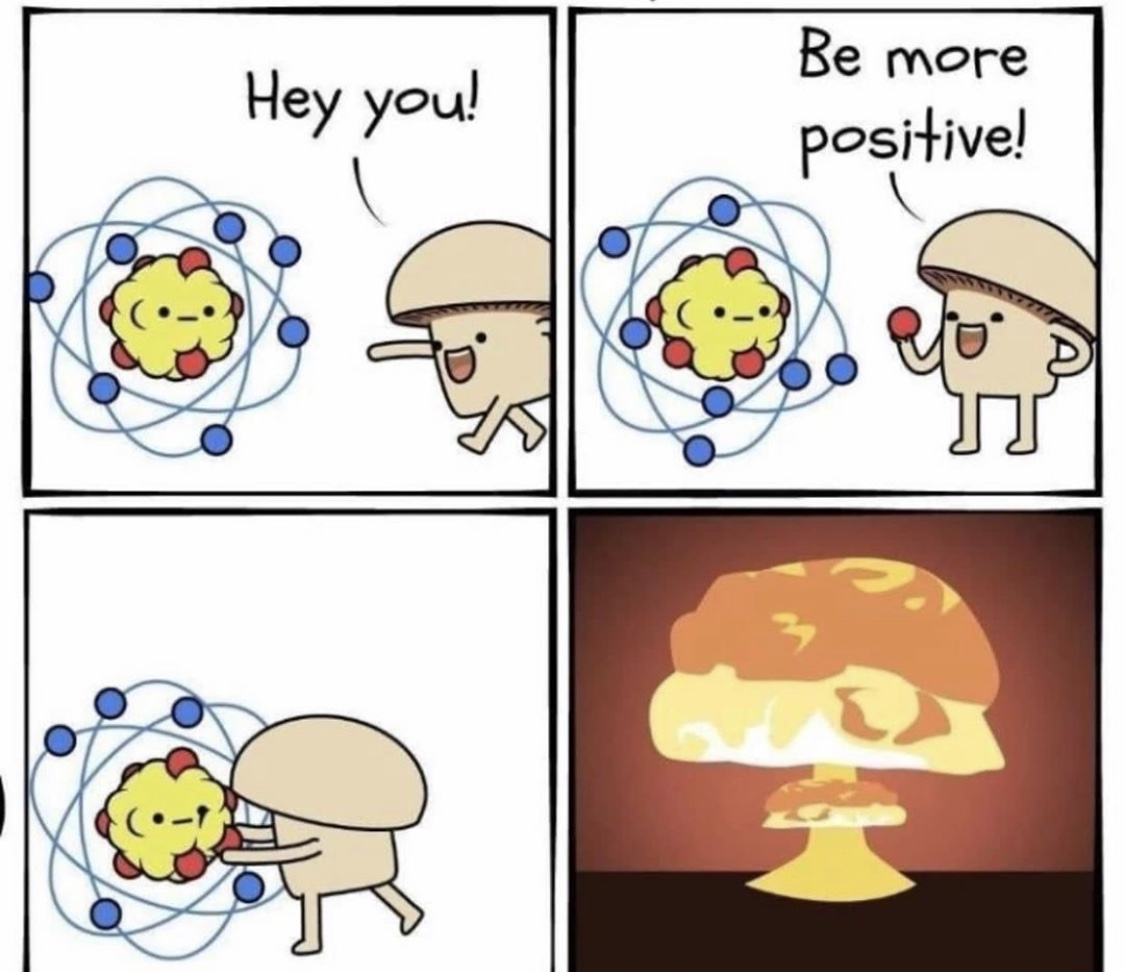
\includegraphics[width=0.8\textwidth,height=\textheight]{fig/positivity.jpg}

Additionally, statistical models that are used to analyze collected data also work under assumptions. For example, a simple linear regression model requires four assumptions:

\begin{verbatim}
- E(y) = Xβ
- Independence
- Equal variance (σ²)
- Normality
\end{verbatim}

Without checking these assumptions, we are using the wrong models and generating misguided insights or misinformation. Thus, relying on models can also have un-intended consequences.

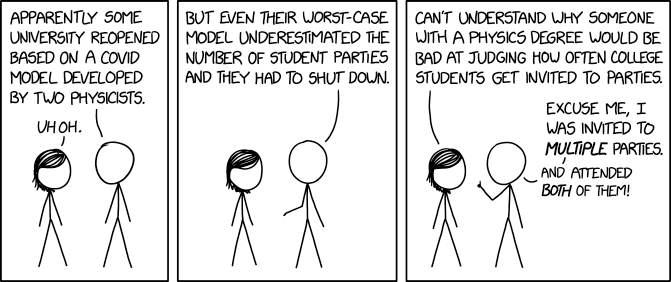
\includegraphics[width=0.8\textwidth,height=\textheight]{fig/modeling_gonewrong.png}

Another instance is not considering degrees of freedom, i.e.~measuring how much information we can get from the data: the more variables are included, the less information is left out but our data analysis models can run out of steam if there are too many variables (problem of big data).

To summarize, experiments can be `dangerous' if we fall into the following pitfalls (not an exhaustive list):

\begin{itemize}
\tightlist
\item
  Devise wrong metrics (i.e.~metrics that don't answer the question at hand)
\item
  Have no clear scope (i.e.~what are the boundaries for the `system under test')
\item
  Omit assumptions and limitations of study
\item
  Use unrepresentative metrics, have no comparison groups, or have cross-contamination
\item
  Not recognize the experimental limitations
\item
  Overlook significant parameters that affect the behaviour of a system
\item
  Report average and not variability (fall for tricks of statistics or have no statistics!)
\item
  Have no interpretation of what results mean or overgeneralizing conclusions
\item
  Ignore errors and outliers
\item
  Not consider the ethical issues and scenarios or have informed consent from participants
\end{itemize}

\hypertarget{it-is-not-all-bad}{%
\section{It is not all bad}\label{it-is-not-all-bad}}

\begin{quote}
Evidence-based policy making can be a political ideal
\end{quote}

Experimentation is not all bad news. Many breakthroughs and transformations on many fronts from medicine and technology to social changes for good have come about by a willingness to experiment. For example, the following:

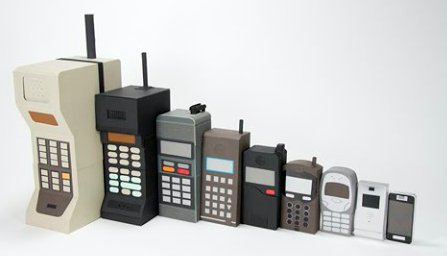
\includegraphics[width=0.8\textwidth,height=\textheight]{fig/cellphone_evolution.png}

There are also many pros to experimentation. For instance, experiments can result in a higher degree of internal validity. Through random assignment of a treatment condition, experimental designs allow us to examine the effect of one variable while keeping other conditions constant. Note that randomization is the key here because it ensures that the treatment and control groups are comparable. Any differences between the two groups can be attributed to the treatment. This is great to know and invest in as a business.

Experimentation can be good even without prior knowledge. This is because sometimes there may not be a theory or theories may fall short to start with. Since an experimentation can directly control how data is generated, the experimental approach can survive and thrive with no previous knowledge. For instance, with no prior knowledge, electoral researchers can carry out a field experiment to examine how different ways of contacting voters would affect the voting turnout.

Experimentation can help clarify mixed results. This is sometimes inherent in observations that are looking at similar phenomena with different measurements or with different data sources. Observational studies often generate mixed results and one way to validate or clarify the existing mixed result is to run an experiment. Again with the example of electoral politics, researchers can chose to run an experiment to detect how campaign spending affects the voters for the incumbent and the challengers differently.

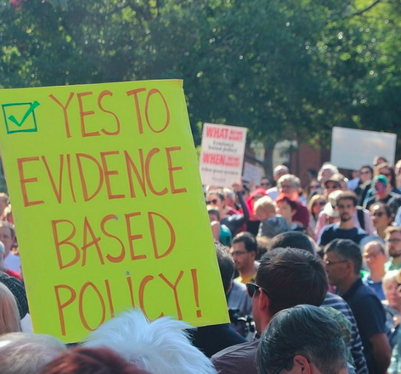
\includegraphics[width=0.8\textwidth,height=\textheight]{fig/march4science.png}

\hypertarget{communication-of-intent-to-experiment}{%
\section{Communication of intent to experiment}\label{communication-of-intent-to-experiment}}

Given that we are considering the option to experiment, we need to have clear and open communications and collaborations with cross-functional teams.

The aim is to get feedback from as many diverse people as possible. These conversations can not only help us decide which ideas to take forward, but also reiterate clear questions based on feedbacks, and eventually implement in an experimentation proposal.

These conversations presumes that there is already an executive level buy-in in place and that stakeholders are invested in the experimentation process. This also assumes that a clear and thoughtful design and implementation plan exists before starting to communicate such that it can be communicated wholly and incrementally with the executives. This is not a tautology and hopefully drive the point that iteration, re-iteration, agility, and an open attitude are key qualities in the initial process.

Executive buy-in usually requires a thorough risk assessment and contingency plans more so in the public service space than in academic environments. Therefore, it is important that the executive is aware of the experimentation cycle which can also be thought of as the problem-solving process and endorses the method, approach, tests, and tools that generate evidence. Some, in fact, argue that experimentation is the creation of something new in the face of uncertainty and risk.

\begin{quote}
It is noteworthy that the word ``experimental'' has come to mean ``innovative'' or ``radical'' rather than simply ``untested''. \href{A\%20catalogue\%20of\%20experiments\%20for\%20decision-makers\%20and\%20professionals}{The Experimenter's Inventory}
\end{quote}

Genuine experimentation is about committing to rigorous assessments and evaluation of evidence, not just freewheeling ``trying stuff out'' or doing things differently and expecting to succeed.

Therefore, even though a methodology is key to answering a specific question, the starting point is having a problem you are trying to resolve, preferably with the social good in mind. The purpose of experimenting is to test key questions and assumptions using quick, low risk experiments.

From the thousands of experiments conducted by Thomas Edison to create the first lightbulb, or the long-running field experiments by Gregor Mendel to examine genetic variability that today underpins modern agriculture concepts, through to trials in medicine, carefully testing ideas in practice is a cornerstone of scientific and technological discovery.

\hypertarget{experiments-in-the-public-sphere}{%
\section{Experiments in the public sphere}\label{experiments-in-the-public-sphere}}

Today, experiments are critical to sectors where innovation and optimization are routine, such as web development, digital transformation, electrical vehicles, etc. This has caught on in business such that the largest financial institutions, retailers and restaurants are also running randomized experiments, along with companies like Google, Facebook, and Amazon running tens of thousands of experiments a year. A/B testing is now the standard means through which Silicon Valley improves its online products. However, in government experimentation remains relatively rare and a new field.

A small but growing movement of policy experimenters are bringing fresh ideas on how to solve public problems. From crafting better services, to making the back-office of government more efficient, new methods and tools need to be used to develop and test policy. In fact, government must rigorously and systematically put policy to the test -- or risk stagnation.

\begin{verbatim}
In the context of government agencies, experiments aim to evaluate a program, policy, 
or service and test an idea or innovation by investigating what difference it has 
made or will make for the people it is aiming to help. 
\end{verbatim}

Like laboratory experiments, public sphere experiments also need a control group to test an innovation against ``business-as-usual''. This doesn't have to be a large trial like testing a drug and can be fast and flexible. In fact, the best experiments start small and as a prototype before they are extended.

For example, the World Bank advocates for ``nimble randomized control trials''. They funded nimble evaluations on how best to improve the take up of health insurance in Azerbaijan, expand the use of contraceptives in Burundi, and support teachers to deliver tailored education to children affected by war and displacement in Lebanon.

\hypertarget{summary-deciding-to-experiment}{%
\section{Summary: deciding to experiment}\label{summary-deciding-to-experiment}}

\begin{itemize}
\tightlist
\item
  Do you need to experiment? Why or why not?
\item
  Find a behaviour, program, policy, or service to test
\item
  Try out of the box thinking to brainstorm, make observations
\item
  Look for natural experiments
\item
  Talk to experts and get feedback
\item
  Think small and short term
\item
  Start with a proof-of-concept question and hypothesis
\item
  Keep it simple and try to test one thing at a time
\item
  Measure everything that matters
\item
  Have control and treatment groups when possible
\end{itemize}

\hypertarget{experiment-components}{%
\chapter{Experiment components}\label{experiment-components}}

\hypertarget{the-problem-statement}{%
\section{The problem statement}\label{the-problem-statement}}

\begin{quote}
Experimentation as a problem-solving process carried out under controlled conditions in order to discover an unknown effect or law, to test or establish a hypothesis, or to illustrate a known law
\end{quote}

Experimentation is described as many things: a method, an approach, a test, or a tool to generate evidence. All of this is true, but experimentation is first and foremost a problem-solving process.

The starting point for your experiment should not be the methodology, nor a predetermined answer; it should be the problem you are trying to resolve.

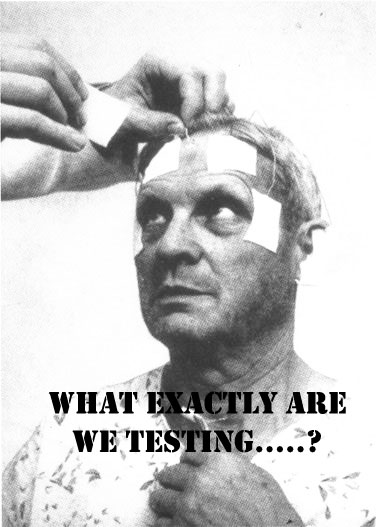
\includegraphics{fig/experiment-meme.jpg}

To help us chose the problem statement, we can go through the following steps:

\textbf{Step 1: Choose a topic}
1. What do I find interesting about the subject?
2. What is known about the subject?
3. What is missing and what are the gaps?

In theory, the topic could be in any field (for instance, agriculture, but also fiscal policy) and at any level (for instance, it could affect 20 people, or it could reach most of Canada's population). It could touch upon the realm of policy, program, service delivery, regulatory and internal services.

The problem doesn't always need to be causal in nature, in which case perhaps an observational study is better.

\textbf{Step 2: Narrow the topic}
1. What do you need to know more about on the topic?
2. Are you interested in social, political, economic, gender, religious issues related to your topic?
- Find a ``slant'' on your topic and determine the root causes (physical, social, or organizational causes)
- Develop possible solutions and select a solution
3. Will the results reveal something new or unexpected?
4. What is in scope and what is out of scope?
5. Can you clearly define hypotheses (If\ldots{}then\ldots{}) and explicitly state research questions?

The problem statement you develop should be clear and precise, but also scoped into a relevant policy area that is within your reach (in terms of jurisdiction, for instance). A problem that has too little impact to be deemed important is likely not a great fit, nor is a problem with little decision-making implications very useful to be explored. Similarly, problem statements that are too vague need to be modified so that they're scoped appropriately.

\textbf{Step 3: Find Resources}
1. How do we design a research proposal that builds on existing knowledge to address critical questions?
2. The key here is getting to know what is already done on the topic and how can our design improve or build on current knowledge.
3. Perform a systematic literature search by using the keywords you have compiled and use them to search for books in Library Catalogs, blogs, or articles in online databases
4. Consult with experts and seek feedback

In a government context, the right scale and scope of the experiment will be dictated by what decision-makers need to know coupled with the various practical constraints that inevitably come along through the design process.

In general, this step will help us make the proposal more mutually exclusive and collectively exhaustive, \textbf{MECE}. By the end of this process, more so that before, we will be able to make statements that do not overlap in content and fully describe the problem at the highest level.

\textbf{Step 4: Seek collaboration}
1. Make sure the question is one that other people can get behind and support
2. Establish collaboration agreements and executive buy-in
3. Peer-review for clarity, scientific accuracy, and feasibility
4. Does the team have the expertise required to complete the project? If not, who else needs to be on team

Figuring out the problem will take time, and needs to be done in consultation with as many parties directly or indirectly potentially impacted by the experiment's results. Before starting the problem definition stage, you should take time to discuss alongside colleagues, management and others (experts and practitioners, current users) what exactly you wish you fix.

Each of the steps above should be completed before moving on to the next one. However, steps can be repeated. For example, if you're on the third step, you can still return to the previous step, and redefine the problem.

\hypertarget{determine-interventions}{%
\section{Determine interventions}\label{determine-interventions}}

It's important to be clear what the different experimental designs can and can't tell us. What sets observational studies apart from experimental studies is that there is a component of \textbf{intervention} in experimentation.

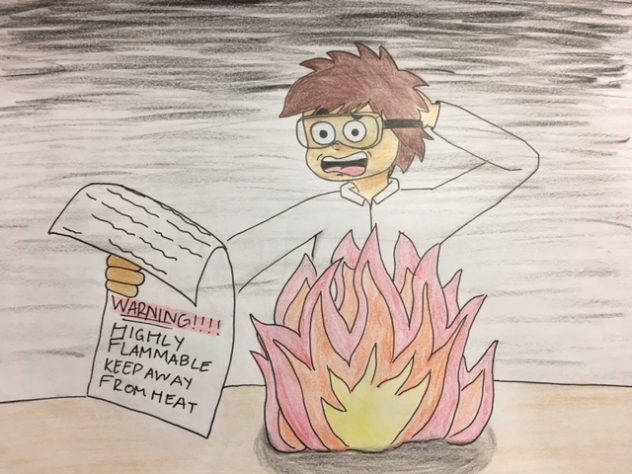
\includegraphics{fig/experimentation.jpg}

Only certain experimental designs are helpful for learning about impact and effectiveness of an intervention. Therefore, we need to select a design that best tells us whether or not our new idea is really making a difference. This approximates a controlled experiment of basic science.
When setting up an experimental design, we need to think about what the intervention (treatment) might look like in our program/ operation. It is helpful to think of interventions as steps that help us evaluate the direct impacts of treatment or preventive measures on a situation.

When thinking about interventions, it is helpful to consider the two following points:

\textbf{Deciding what to measure}: using a government contractor example, consider what kind of data you'd need to answer your key question. In this case, you'd need to know the number and cost of current staff and the percentage of time they spend on necessary business functions. In answering this question, you likely need to answer many sub-questions (e.g., Are staff currently under-utilized? If so, what process improvements would help?). Finally, in your decision on what to measure, be sure to include any reasonable objections any stakeholders might have (e.g., If staff are reduced, how would the company respond to surges in demand?).

\textbf{Deciding how to measure it}: thinking about how you measure your data is just as important, especially before the data collection phase, because your measuring process either backs up or discredits your analysis later on. Key questions to ask for this step include:
- What is your time frame? (e.g., annual versus quarterly costs)
- What is your unit of measure? (e.g., USD versus Euro)
- What factors should be included? (e.g., just annual salary versus annual salary plus cost of staff benefits)

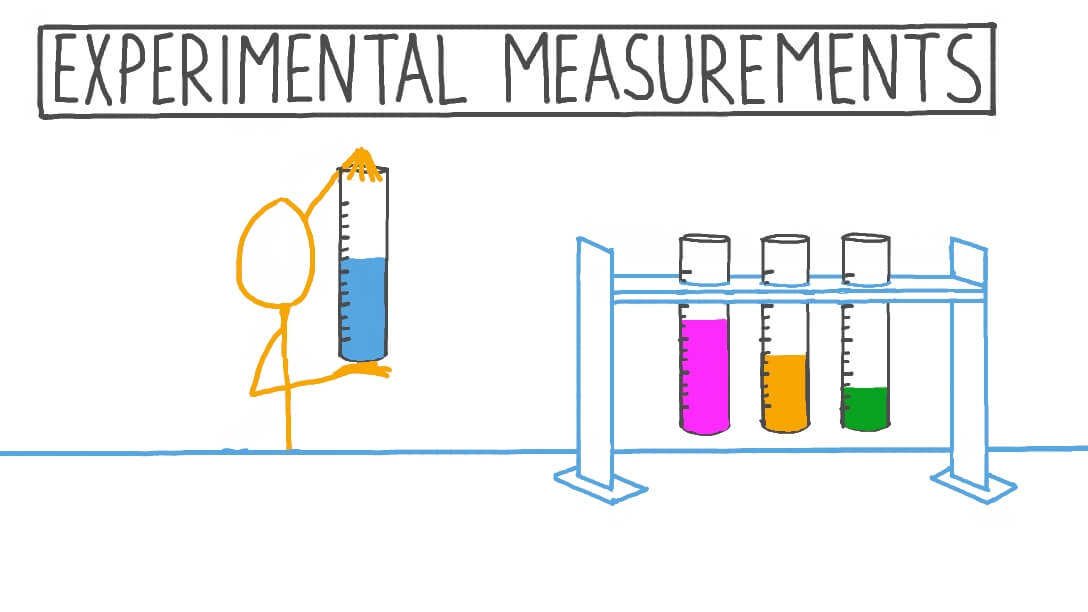
\includegraphics{fig/experimental_measurements.jpeg}

\hypertarget{determine-outcomes}{%
\section{Determine outcomes}\label{determine-outcomes}}

When designing the intervention, it is also important to determine what you want to measure and what the hypothesized effects might be. This will illuminate what data we need to collect, set targets, and develop counter-measures. As part of this, we would want to identify the techniques we will need to perform the measurements and use the collected data for analysis.

An outcome measure, endpoint, effect measure or measure of effect is a measure which is used to assess the effect, both positive and negative, of an intervention or treatment. Measures can often be quantified using effect sizes. They can also be thought of as providing a score, an interpretation of results or at times a risk categorization of study groups. Prior to providing any intervention, an outcome measure provides baseline data on variable.

Also of note is that experimental studies are usually randomized, meaning the subjects are grouped by chance and we study what happens to people in each group (treatment and control). Any difference in outcomes can then be linked to the intervention.


\includegraphics{fig/RCT-graphic.png}

For instance, a well designed randomized control trial (RCT) provides a strong evidence that a given intervention can postulate effectiveness or safety. A RCT is best used when we need to draw conclusions on causality but there are many other experimental designs we can draw on and this will be discussed in Module 3.

\begin{quote}
It helps to think of outcome measures through visualization of outcomes / prototypes
\end{quote}

As well as increasing our understanding of what experimental design to use when, there is scope for experimenters to get much better at using different tools in combination to innovate more effectively. Prototypers, for instance, could use low-cost randomized trials like A/B tests or nimble trials to evaluate prototyped products or services.

Prototyping emphasizes front-loading risk and creating a solution with a better chance of success through stakeholder engagement. Using plastic Lego bricks to build prototypes of engineering products is a low-fi, low-resource way of making early operational or design issues obvious. But it won't tell you whether or not the new system works in real life, or at scale.

When designing prototypes, we should think of implementing an intervention to measure the outcomes. For this, we need an independent variable or the factor that is manipulated, changed, or intervened. This is usually a variable that is placed on x-axis when grouping. We also need a dependent variable or the factor that is being measured and usually placed on y-axis during grouping and visualization.

\hypertarget{experimental-designs}{%
\section{Experimental design(s)}\label{experimental-designs}}

Next is to determine if randomization is possible, what the sampling unit and approach might be, how the control group might be set up as well as how many observations are needed based on power calculations.

Randomized experiments, or quasi-experimental designs, sometimes couched in deadly technical language, are uniquely valuable. Despite their unfashionable status among some policy wonks and evaluators, we will also highlight the value and utility of Quasi-Experimental designs in the next module. Other approaches may be also be suited to finding out different things, at different stages of developing a policy solution.

Regardless of what type of experiment we chose to do, it is helpful to think about the following variables:

\begin{itemize}
\tightlist
\item
  A control group is a group of `test' items in an experiment. The control group will be used to compare with the experimental group
\item
  The control group doesn't get the treatment
\item
  An experimental group is the group(s) of test items where only one change (called the experimental or independent variable) has been made
\item
  The experimental group gets the treatment
\item
  The experimental group may have dependent or independent variables
\end{itemize}

In the case when a real control group is not available, a synthetic control group or a more inventive statistical methods may be useful.

It is also in this step that we determine what information we want to collect, set a timeframe for data collection, and determine the data collection methods.

\textbf{Source of error considerations}
- Mind the constants: the conditions that are kept the same for control and experimental groups
- Not controlling for factors or parameters that are kept the same in both control and experimental groups can result in error
- Type I error (α) is the rejection of a true null hypothesis (\emph{``false positive''} finding or conclusion, e.g. ``an innocent person is convicted'') or finding a difference when a difference does not exist
- Type II error (β) is the non-rejection of a false null hypothesis (\emph{``false negative''} finding or conclusion, e.g.~a guilty person isn't convicted) or not detecting a difference when one actually exists

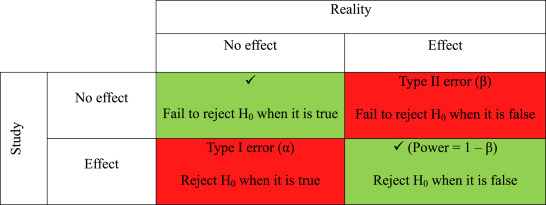
\includegraphics{fig/null.jpg}

\textbf{Sample size considerations}
Sample size measures the number of individual samples measured or observations used in a survey or experiment. For example, if you test 100 people for COVID, your sample size is 100.

In general, we want to:
- Maximize sample size (n): the larger the number of test items the more accurate the estimate
- Use representative groups: the samples must reflect the natural variation in the population.
- Use random or systematic sampling to reduce inherent bias in data.

For sample size calculations, we need a hypothesis test, a significance level for the test, the smallest effect size (∆) that is of scientific interest, and the intended power (power = 1 -- β) of the test.

There are often softwares that help statisticians decide what sample size and power to chose for a set of sample observations. In general:
- The price of increased power is that as standard deviation goes up, so does the probability of a Type I error because
- As sample size increases, so does the power of the significance test. This is because a larger sample size narrows the distribution of the test statistic

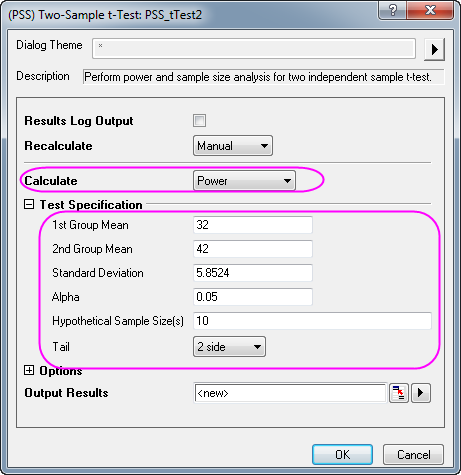
\includegraphics{fig/samplesize.png}

Statistical power is a measure of the likelihood that a researcher will find statistical significance in a sample if the effect exists in the full population. Power is a function of three primary factors: sample size, effect size, significance level.

\hypertarget{collect-and-analyze-data}{%
\section{collect and analyze data}\label{collect-and-analyze-data}}

At this point, we have a problem, and intervention, a research plan, and data collection strategies. Therefore, we are ready to start implementing the experimental design to collect the data and then analyze it.

We can treat data as qualitative (descriptive) or quantitative (quantitative values/ numbers). Before you collect new data, determine what information could be collected from existing databases or sources on hand. Collect this data first. Also determine a file storing and naming system ahead of time to help all tasked team members collaborate. This process saves time and prevents team members from collecting the same information twice. If you need to gather data via observation or interviews, then develop an interview template ahead of time to ensure consistency and save time. Keep your collected data organized in a log with collection dates and add any source notes as you go (including any data normalization performed). This practice validates your conclusions down the road.

\textbf{Quantitative data} comes in the form of numbers, quantities and values and describes things in concrete and easily measurable terms. Examples include the number of students who applied to a grant, the rating a customer gave a product out of five stars and the number of times a visitor spent on the website.

\textbf{Qualitative data} is descriptive, rather than numeric. It is less concrete and less easily measurable than quantitative data. This data may contain descriptive phrases and opinions. Examples include an open ended review a customer writes about a product, an answer to an survey question about what type of applications a customer likes to fill and the conversation an applicant has with a service representative.

Regardless of what kind of data we collect, a proactive data management strategy will make storage, retrieval, and analysis easier.

The analysis phase is also as crucial because it turns raw data into valuable insights that we can use to enhance strategies, products and business decisions. We can often couple data analytics tools to raw data (e.g.~power BI softwares, etc) to help with analysis. Visio, Nvivo, Minitab, Stata, and Microsoft Excel are other great tools and software packages for advanced statistical data analysis. The goal of analysis of the data to really to test the effects of the intervention we wanted to measure (e.g.~comparing the differences between groups who got a treatment and those who didn't).

Devote some time to review the results. What happened after you implemented the interventions? What worked, what didn't, and what did your solution improve? Analyze if your actions made the required impact and if you addressed the root causes of the issue. It's also time to look for improvements in the solution and to plan ongoing monitoring. You can also analyze what you've learned and what still needs to be learned when it comes to problem-solving processes and skills.

As you interpret the results, ask yourself these key questions:

\begin{itemize}
\tightlist
\item
  Does the data answer your original question? How?
\item
  Does the data help you defend against any objections? How?
\item
  Are there any limitation on your conclusions, any angles you haven't considered?
\end{itemize}


\includegraphics{fig/data-analysis.jpg}

Once you have uncovered the patterns and insights, you can start reporting back the findings to stakeholders. This step is also reiterative because as you report back, you can adapt the information. Through the presentation of the results, you disseminate the evidence that identities key learnings and adapt the program/ operation based on what the evidence dictates.

The goal of sharing the results and reporting back the process to executives is to reach consensus, generate additional learnings, and develop a better implementation plan.

\textbf{Problem-solving tips}

Problem-solving is a process of constant improvement and reiteration. Don't expect the perfect solution from the start or that the problem won't appear in the future. We should make efforts not to avoid problems because they're part of the learning process. If you adopt an attitude in which you focus on finding solutions every time new challenges emerge, you'll save yourself a lot of time and stress.

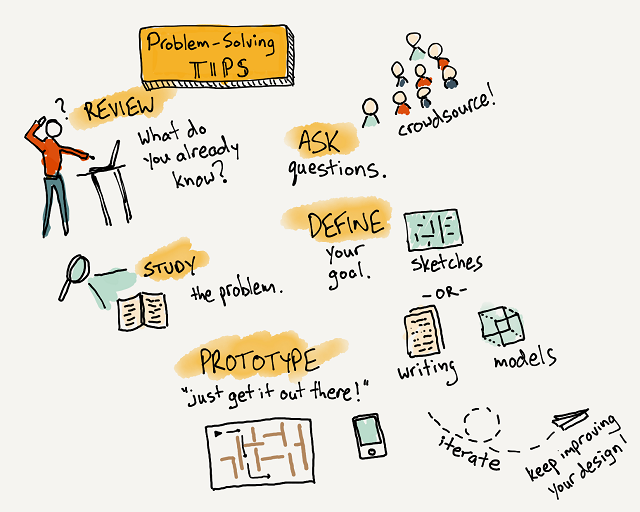
\includegraphics{fig/tips.png}

\hypertarget{mechanics-of-endorsement}{%
\chapter{Mechanics of endorsement}\label{mechanics-of-endorsement}}

\hypertarget{knowledge-co-production}{%
\section{Knowledge co-production}\label{knowledge-co-production}}

Communicating the project with intention to gain the trust and cooperation of project team is an imperative step prior to starting an experimentation process. More and more, we are moving towards knowledge co-production models as one person isn't capable of delivering complex multi-faceted projects. To achieve co-production, clear and intentfull communications with team members can affect the success of the project. Buy-in can be difficult to quantify, especially within various stakeholder categories. However, without full buy-in from team members, sponsors and other stakeholders, projects may seem to be progressing smoothly and then suddenly take a sharp turn for the worst, risking the final deliverables and team satisfactions.

Below are the main steps for sustainable co-production research.

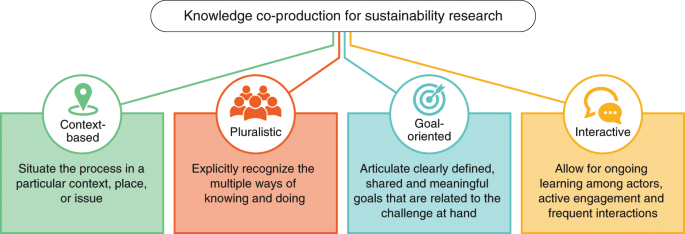
\includegraphics{fig/team-co-production.png}

To improve communication with team members at each stage of a project and to make sure they feel like an important part of a team, the following points may be helpful:

\begin{enumerate}
\def\labelenumi{\arabic{enumi}.}
\tightlist
\item
  Identify what motivates the project team and each member individually
\item
  Focus on telling the truth about the project, even when it isn't what team members want to hear
\item
  Make sure all team members understand their contribution to the project
\item
  Reaffirm goals and communicate progress throughout execution
\item
  Remain consistent
\item
  Provide positive feedback throughout the process and after the project ends
\end{enumerate}

\hypertarget{executive-buy-in}{%
\section{Executive buy-in}\label{executive-buy-in}}

Once an experimentation plan has been devised, you will need to make a good case as to why the strategy deserves a dedicated budget and resources and what sets this apart from other program initiatives already in place.

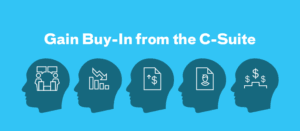
\includegraphics{fig/buy-in.png}

So how do you do it? Below are 3 steps to help in making a convincing case to obtain executive buy-in for your proposal.

\begin{enumerate}
\def\labelenumi{\arabic{enumi}.}
\item
  Figure out who you should be talking to, that is, identify the relevant stakeholders in your organization who have the authority to sign off on a new strategy, allocate budget resources and designate personnel. You can make a list of the people you want to target. Next, you can ask what business needs do they face and what problems does the organization have that an experimentation can solve? Think like a marketer present your plan as a solution to those specific problems. It is also helpful to find a personal advocate within the organization to function as a change agent---someone who believes in you and has enough clout to advocate on your behalf. This will help give your experimental plan some authority when you present it to the executives.
\item
  Show your accomplishments and what the experimentation can do. This precludes getting to know your organization's analytics capacity and correlating your experimentation success with the real results already existing. For instance, you can communicate that ``you have been doing X, and it's been contributing to Y''. Evidence-based plans are a powerful formula for getting executive buy-in. What if your community is relatively new, or not yet in existence? If this the case, you can benefit from the experience of others and researching a cache of other success stories ready to be applied to your programs. The question the executives will want to know is, how will you make another's success your own success. This requires an experimentation plan.
\item
  Lay out the experimentation's strategic plan for success. Once you have identified key stakeholders and worked on a compelling vision of how you can solve a key problem, you can start sharing that strategic plan. Your plan should, at a minimum, answer the following questions:
\end{enumerate}

\begin{itemize}
\tightlist
\item
  What specific actions must you take to build a community for your research plan?
\item
  What resources do you need to take those actions?
\item
  What results---concrete and abstract---do you hope to achieve?
\item
  What are the risks? how are the risks managed?
\item
  How will you measure your results against your actions?
\item
  How will you quantify the value of this process?
\item
  Are your expectations realistic? Prove it.
\item
  What are your performance deadlines?
\end{itemize}

\hypertarget{communication-matrix-tips}{%
\section{Communication matrix tips}\label{communication-matrix-tips}}

Communication of the intent to experiment and the experimentation processes is like an onion. We can start in the inner layer with peers and colleagues and close supporters who can understand the message. From there, your secondary networks help build momentum. Once it's clear your science resonates with people, then you can reach a larger audience such as the executive or to press and media.

To relay the necessary information about the experimentation plan to stakeholders/executive and to reach consensus, the following points can be considered:

\begin{itemize}
\tightlist
\item
  Why do we need to answer this scientific question now? (\emph{importance})
\item
  Has this question been answered? Has it been attempted? (\emph{novelty})
\item
  What's the risk, and what's the potential upside? (\emph{impact})
\item
  Is the design of the experiment sound? how? (\emph{design})
\item
  What are the timelines and milestones? (\emph{logistics})
\item
  What makes this researcher/research team uniquely qualified? (\emph{qualifications})
\end{itemize}

\hypertarget{code-of-ethics}{%
\section{Code of ethics}\label{code-of-ethics}}

Concerns about misinformation and the inability to distinguish the contrived from the authentic is growing be it in journalism, marketing, finance, or medicine.

Unlike traditional \emph{observational} methods where one makes observations about the world, the \emph{experimental} approach learns about the world by measuring how it reacts to interventions. Experimental studies raise a host of ethical concerns that social scientists are not always well equipped to deal with. The absence of clear principles to handle complex issues and address ethical implications and unintended consequences can leave teams in a difficult situation, above and beyond whether they receive formal research approval.

There are, however, opportunities to experiment even on difficult social issues such as interventions in poverty policies, drug use, or healthy-living interventions. Creating a control group can carry its own risk. If, for example, we are experimenting with a new benefits scheme, having a control group allows us to test whether the scheme has actually achieved its goals, but it also means depriving a group of citizens of an improved service, at least initially.

Broadly, ethical concerns can fall into the problem of \textbf{audience} (what are the issues), \textbf{agency} (who is responsible for interventions), and \textbf{consent} (are participants informed and do they consent). Some other points to consider include the following:

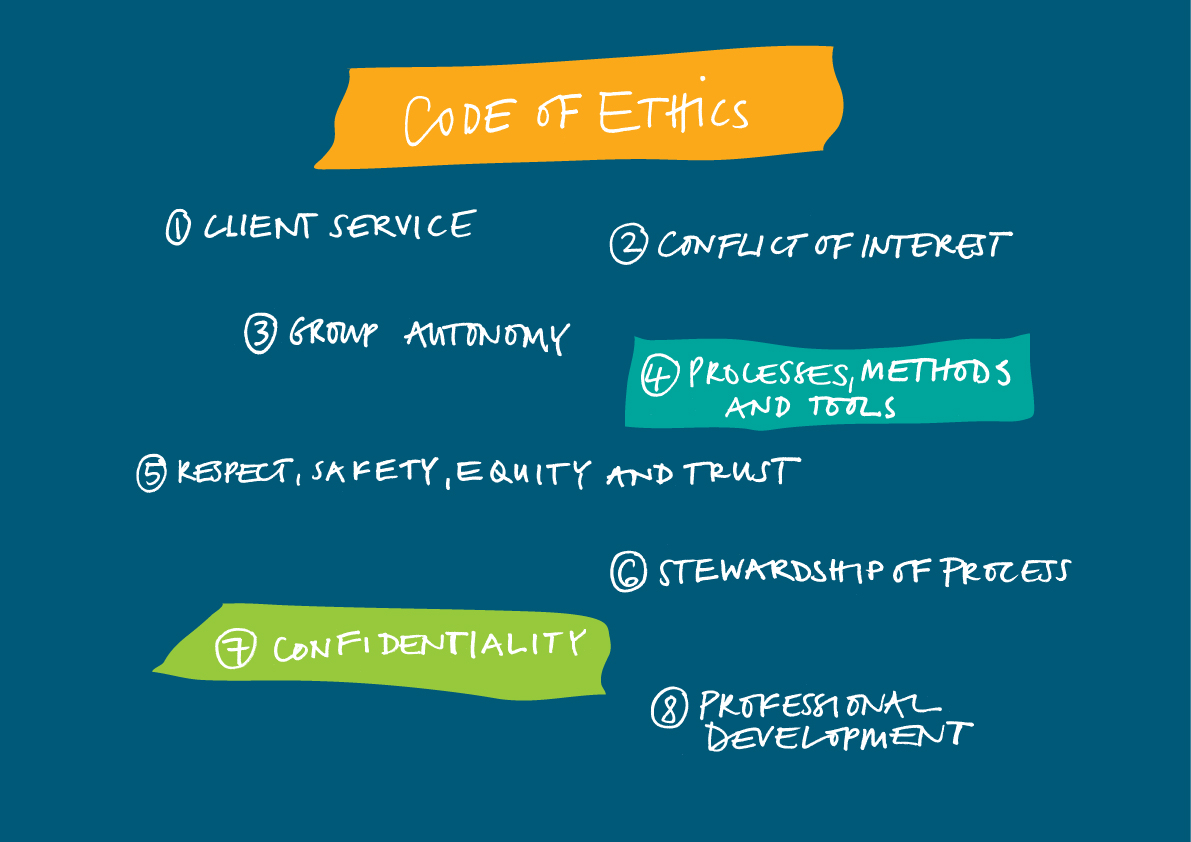
\includegraphics{fig/CodeOfEthics.jpg}

To get around this, a phased policy roll-out can create what's called a ``waiting list'' experiment where the control group are the soon-to-have-innovation group. Everybody eventually receives the new policy innovation, negating the risk of push-back from the public. This approach was used by the UK's Ministry of Housing, Communities and Local Government in their first ever randomized trial on community integration. In 2016, they tested whether English language training could help immigrants engage more in their community.

The results were impressive. They found significant improvements on many social integration outcomes, such as new friendships formed with people from other cultures, and attending more health appointments. The trial helped the Department put together new plans for their 2018 Integrated Communities including a network of conversation clubs and a new English language fund.

Ethical considerations:
- Inform users and the study population and get consent of participation
- Establish information sharing agreements and memorandums of understanding
- Identify situations where experimentations are appropriate and relevant
- Perform privacy impact assessments/agreements
- Get ethics committee approvals
- Check Institutional Review Board (IRB) approval requirements prior to the launch of the experiment

\hypertarget{case-study}{%
\chapter{Case study}\label{case-study}}

For illustration purpose, we are going to use a contentious example. Following the 2016 U.S. presidential election, many have expressed concerns about the effects of false stories, \emph{``fake news,''} as it has been dubbed, circulated largely through social media on the election results.

Many have speculated that the exposure to fake news has shaped people's political inclinations in the presidential election. This group argue that the falsified information delivered in a such dramatic way shifts political inclinations. Others, however, argue that consumption of information is more of a selection process: voters choose their sources of political information on the basis on their existing political preferences. As a result, fake news only reinforces the voters' results but will never change their beliefs.

\hypertarget{background-research}{%
\section{Background research}\label{background-research}}

Recent evidence shows that:

\begin{enumerate}
\def\labelenumi{(\arabic{enumi})}
\tightlist
\item
  62\% of US adults get news on social media (Gottfried and Shearer 2016)
\item
  the most popular fake news stories were more widely shared on Facebook than the most popular mainstream news stories (Silverman 2016)
\item
  many people who see fake news stories report that they believe them (Silverman and Singer-Vine 2016)
\item
  the most discussed fake news stories tended to favor Donald Trump over Hillary Clinton (Silverman 2016)
\end{enumerate}

Putting the above observations together, a number of commentators have suggested that Donald Trump would not have been elected president were it not for the influence of fake news (for examples, see Parkinson 2016; Read 2016; Dewey 2016).

\hypertarget{the-problem-statement}{%
\section{The problem statement}\label{the-problem-statement}}

Did fake news affect the election result by making it more difficult for voters to infer which electoral
candidate they prefer?

Hypothesis: Fake news is independent of election outcome

\hypertarget{scenarios}{%
\section{Scenarios}\label{scenarios}}

In this example, there are three potential causal relationships.

\textbf{1. Fake news affects voting}: Fake news carry certain pieces of information in a way that changes audiences' preferences.

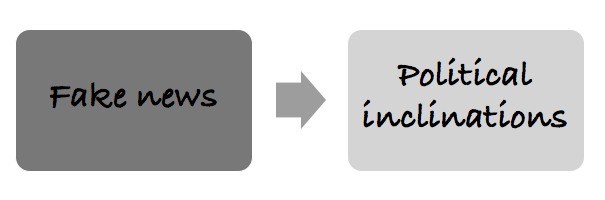
\includegraphics[width=0.8\textwidth,height=\textheight]{fig/scenario1.png}

\textbf{2. Political affiliations determine consumption of news}: People with certain preferences and orientations choose to watch fake news. So, fake news only reinforces but won't change the existing beliefs.

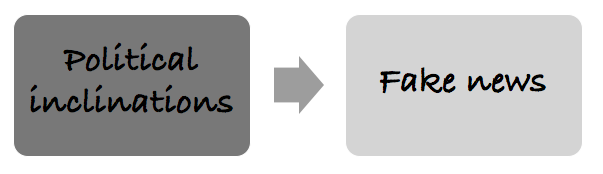
\includegraphics[width=0.8\textwidth,height=\textheight]{fig/scenario2.png}

\textbf{3. Two-way causation}: Political preferences determine which pieces of political information to receive. In turn, it further shapes the existing preferences and changes voters' behaviours. To test these scenario, we can apply a simple experimental design and test it.

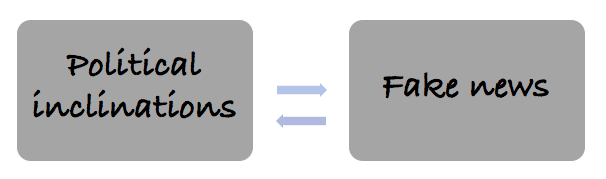
\includegraphics[width=0.8\textwidth,height=\textheight]{fig/scenario3.png}

\hypertarget{experimental-solution}{%
\section{Experimental solution}\label{experimental-solution}}

\textbf{Stage one}: Recruit and randomly assign participants into treatment and control groups; pre-test.

\textbf{Stage two}: Expose the treatment group to fake news; apply placebo to the control group.

\textbf{Stage three}: Record the results of the treatment and control groups. Due to the randomization process, we can control for any previous differences between the treatment and control groups. Therefore, any differences between Result 1and Result 2 are attributable to the presence of fake news.

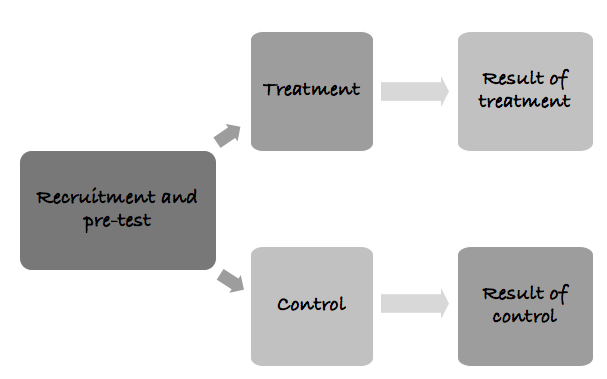
\includegraphics[width=0.8\textwidth,height=\textheight]{fig/stage1.png}

\hypertarget{references}{%
\chapter{References}\label{references}}

\begin{itemize}
\item
  \href{https://vancouver.ca/files/cov/navigating-complexity-solutions-lab.pdf}{City of Vancouver Solution Lab's Principles of Experimentation}, adapted from \href{https://www.nesta.org.uk/toolkit/playbook-for-innovation-learning/}{Nesta's Innovation Playbook}
\item
  \href{https://media.nesta.org.uk/documents/Nesta_CompetencyFramework_Guide_July2019.pdf}{Nesta's Competency Framework for Experimental Problem Solving}
\item
  \href{https://states-of-change.org/assets/images/StatesofChange_Curriculum_Craft.png}{States of Change's Core Elements of Innovation}
\item
  \href{https://gww.gov.bc.ca/sites/default/files/group/file/2019/0207/remixtatyanamamutleadingacultureofinnovationlowres.pdf}{Tatyana Mamut's eight Innovation Elements}
\item
  \href{https://info.themoment.is/innovationculture}{The Moment's Culture Scan}
\item
  \href{https://cdn2.hubspot.net/hubfs/3903042/themoment_InnovationDesignersCapabilityMap.pdf}{Innovation Designer Capability Map}
\item
  \href{https://www.alliance4usefulevidence.org/}{Alliance for useful evidence}
\item
  \href{https://www.alliance4usefulevidence.org/publication/better-public-services-through-experimental-government/}{Better public services through experimental government}
\item
  \href{https://www.gov.uk/government/publications/cross-government-trial-advice-panel-role-and-membership}{The What Works Trial Advice Panel}
\item
  \href{https://www.gov.uk/government/consultations/integrated-communities-strategy-green-paper}{Integrated Communities Strategy green paper}
\item
  \href{https://assets.publishing.service.gov.uk/government/uploads/system/uploads/attachment_data/file/495329/The_impact_of_Sure_Start_local_programmes_on_7-year-olds_and_their_families.pdf}{The impact of Sure Start Local Programmes on seven year olds and their families}
\item
  \href{https://assets.publishing.service.gov.uk/government/uploads/system/uploads/attachment_data/file/786891/National_evaluation_of_the_Troubled_Families_Programme_2015_to_2020_family_outcomes___national_and_local_datasets_part_4.pdf}{National Evaluation of the Troubled Families Programme 2015 - 2020}
\item
  \href{https://pubs.aeaweb.org/doi/pdfplus/10.1257/jep.31.2.211}{Social Media and Fake News in the 2016 Election}
\item
  \href{https://www.degruyter.com/view/journals/jgd/6/1/article-p87.xml}{Reflections on the Ethics of Social Experimentation}
\end{itemize}

\end{document}
